\documentclass[twoside,11pt]{article}

% Any additional packages needed should be included after jmlr2e.
% Note that jmlr2e.sty includes epsfig, amssymb, natbib and graphicx,
% and defines many common macros, such as 'proof' and 'example'.
%
% It also sets the bibliographystyle to plainnat; for more information on
% natbib citation styles, see the natbib documentation, a copy of which
% is archived at http://www.jmlr.org/format/natbib.pdf

\usepackage{jmlr2e}
\usepackage{amssymb}
%\usepackage{amsmath}
\usepackage{mathtools}
\usepackage{graphicx}


% Definitions of handy macros can go here

\newcommand{\dataset}{{\cal D}}
\newcommand{\fracpartial}[2]{\frac{\partial #1}{\partial  #2}}

% Heading arguments are {volume}{year}{pages}{submitted}{published}{author-full-names}

%\jmlrheading{1}{2000}{1-48}{4/00}{10/00}{meila00a}{Marina Meil\u{a} and Michael I. Jordan}

% Short headings should be running head and authors last names

%\ShortHeadings{Inverse RL in Sepsis Management}{SS, DH and YZ}
\firstpageno{1}

\begin{document}

\title{Learning Intermediate Rewards for Sepsis Management policies using Inverse Reinforcement Learning}

\author{\name Srivatsan Srinivasan \email srivatsansrinivasan@g.harvard.edu \\
       \AND
       \name Linying Zhang \email zhangly811@gmail.com \\
       \AND
       \name Donghun Lee \email donghunlee@g.harvard.edu \\
       }
\editor{}
\maketitle

\begin{abstract}%   <- trailing '%' for backward compatibility of .sty file
Apprenticeship Learning/ Inverse Reinforcement Learning considers learning in a Markov Decision process where an explicit reward function is not given for each action, but the agent is expected to learn from an expert's demonstration of the task. This approach is extremely useful in applications where it may be difficult to write down an explicit reward function underscoring the trade-off across different desiderata. We think of an expert as trying to maximize a reward function expressible as a linear/non-linear combination of known features and provide an algorithm to learn the implicit rewards maximized by the expert. Specifically, we focus on understanding the patient features which act as drivers of clinical policies in sepsis management in ICUs. We compare these features with those learned by an optimal MDP solution. In the process, through the interplay of weights in our reward function approximation, we cast intermediate rewards to states and understand features which maximize and minimize rewards. We would demonstrate that our algorithm terminates in feasible number of iterations and the policy output by the algorithm will attain performance close to that policy we try to learn from.  
\end{abstract}

\begin{keywords}
  Inverse Reinforcement Learning, Apprenticeship Learning, Intermediate Rewards, Markov Decision Process, Sepsis Management
\end{keywords}

\section{Introduction and Related Work}
The process of medical treatment could be considered as sequential interaction between doctors and patients. This setup makes it an ideal candidate for employing reinforcement learning algorithms in order to learn optimal treatment trajectories. The field of reinforcement learning is founded on the presupposition that the reward function, rather than the policy or value function, is the most succinct robust and transferable definition of the task in hand. Unfortunately, in our problem space of sepsis management in ICU, we have time series of patient history and the final tag of survival or demise. The problem setup does not specify any explicit rewards for different state abstractions and it becomes intractable to explain the treatment trajectory of the physicians or the optimal MDP solution. Besides, the data is plagued by sparse and delayed rewards problems. Learning the intermediate rewards from an expert policy provides solid insights into the implicit features that was considered valuable by the expert policy and provides a well-rounded interpretation for the actions suggested by the expert policy. Also, having well-stated intermediate rewards helps in guiding the MDP solution through "good" states more frequently and thus, ensure faster transition to absorbing states - essentially reaping higher Q-value functions.\\[10pt]
The problem of IRL can be formulated as the problem of estimating the reward function of an expert agent who behaves optimally under an environment and the reward function. Several IRL algorithms have been proposed so far. Ramachandran and Emir formulated the IRL problem in Bayesian framework and proposed an algorithm using MCMC sampling[5]. Rothkopf and Dimitrakakis reformulated the Bayesian IRL within the framework of preference elicitation and also extend the method for multitask learning[6]. Ng and Russell proposed an algorithm using linear programming[2].Abbeel and Ng proposed another algorithm employing quadratic programming - "apprenticeship learning" which used the estimated reward function to mimic the behavior of expert agent[1]. In this work, we are going to follow this approach for the first version and later use Bayesian IRL if time permits.

\section{Proposed Algorithm - Discussion of features and challenges }
We start the problem by setting our absorbing states of survival and mortality yielding rewards of +1 and -1 respectively. We assume that there is some vector of features $\phi$ over states and that there is a true reward function $R^*(s) = w^* \cdot \phi(s)$.  In order to ensure that the rewards are bounded, we suggest the use of two different approaches. One approach would be to choose $\phi$ from a power set of binary features and set $||w^*||_2 \leq 1$. Some example features in our problem would include "is gender male" and "has the BP crossed a particular threshold". This approach involves finding binary representations for continuous features which requires good boundary definitions. Another approach is to use the existing features as they are and combine them linearly before applying a squashing function such as $f(x) = tanh(x)$ to curtail the linear approximator's range  to (-1,1). The non-linearity in the latter approach might make the optimization problem intractable in the later stages and we acknowledge the challenges involved in this definition. We propose to start with the former and then dwell into the latter if the former proves insufficient. \\[10pt]
In our data set, we already have access to the demonstrations by some expert, $\pi_E$. Let $D$ be the set of all states. We define feature value vector or more succinctly, \textbf{feature expectations} to be 
\[\mu(\pi) = E[ \sum_{t=0}^{\infty} \gamma^t \phi(s_t) | \pi ] \in \mathbb{R}^k \]
This notation helps us calculate the value of the policy to be 
\[E_{s_o \sim D}[V^{\pi}(s_0)] = w \cdot \mu(\pi)\]
In our problem space, we have several set of trajectories adapted by the experts. We need to setup an appropriate definition of a physician policy in order to calculate the feature vector of the expert policy. We propose to try out multiple variants of inferring physician policy from the data set and we intend to explore each variant in the order of increasing complexity along the course of the project.
\begin{itemize}
\item Choose a population statistic of actions such as median or mode in each state to represent the physician policy.
\item Use supervised learning to infer the physician policy from the history of state actions that employs a latent variable model in order to provide more expression of state characters.
\item Use the off-policy SARSA sampling outlined in the work on deep RL based solution to sepsis management[3]. 
\item Choose the most plausible action from a state that belongs to the closest neighbors of this state in a kernel - an approach we undertook in HW3.
\end{itemize}

Once we have an expert feature expectations, we have all the key ingredients for the setup of the problem. The problem is the following : Given an MDP, a feature mapping $\phi$ and the expert's feature expectations $\mu_E$, find a policy whose performance is close to that of the expert's on an unknown reward function $R^* = w^*{^T}\phi$. To accomplish this, we will find a policy $\hat{\pi}$ such that $||\mu(\hat{\pi}) - \mu(\pi)||_2 \leq \epsilon $. Again, the choice of optimizer is dependent on the setup of the problem. For the initial versions, we propose to use off-the-shelf optimization packages to fetch the initial set of results before dwelling further into this area. \\[6pt]
The algorithm for apprenticeship learning could be outlined thus.
\begin{enumerate}
\item Randomly pick some policy $\pi^{(0)}$, compute $\mu^{(0)}= \mu(\pi ^{(0)} )$ and set the iterator $i$ to 1.
\item Find the $w$ that maximizes $t$ such that $w^T \mu_E \geq w^T \mu^{(j)} + t, \forall j \in [0, i-1]$ subject to the constraints on the $||w||_2$ if any. Intuitively, this step is the inverse RL step where we try to find a reward function $R = w ^{(i)} \cdot \phi $ such that the expected value function of the expert policy does better by a margin of t than the policies visited earlier. Intuitively, because of the L2 norm constraint on $w$, we need to use a quadratic optimizer for this problem.  Another way to think about this is that we are trying to find the maximum margin hyper-plane that separates the expert policy and the policies we have found until now.
\item If $t^{(i)} \leq \epsilon$, then terminate
\item Else using the weights, compute the rewards and solve the MDP to obtain a new policy and its corresponding feature expectation $\mu^{(i)}$.
\item Set $i=i+1$ and go back to step 2.
\end{enumerate}

For the first cut,we are going to leverage an adaptation of the clustering solution for representing the state space we used in earlier homework problems. Improvement of state representation is of paramount importance to this problem and we expect to collaborate with the rest of the groups on obtaining better state representations while ensuring that our code is modular and scalable to adapt to any state representation. \\[10pt]
The overall direction of this project can be broadly defined by three major cornerstones.
\begin{enumerate}
\item Feature engineering - Representing reward functions as a linear combination of data features we have at our disposal would be one of the biggest challenges of this problem. We intend to start off with simple features such as SOFA and employ forward selection approach to add more features to this model.
\item Physician policy - IRL depends on the fundamental assumption that we have an expert policy in play. We have already outlined few approaches that we use to characterize physician policy. Besides,  Characterizing the physician policy is a tricky proposition as we do not have any demarcation within the data which indicates some physician attributes. In the later stages, we can study the distributions of actions for same states by different physicians(Implicit assumption being similar actions from similar states for different patients would mean similar kind of physicians) and apply IRL to a subset of physicians to understand the differences in implicit rewards perceived by different subgroups of physicians. 
\item Theoretical proofs of convergence -  We need to demonstrate the convergence of the aforementioned algorithm and provide $\epsilon$ and probabilistic bounds around our confidence of convergence based on the perceived physician policy.
\item MDP solver - We need a fast MDP solver in order to save large amounts of computation time as the optimization procedure would span several episodes of the MDP. We can try both model free and model based learning and are willing to compromise marginally on the model accuracy for computational efficiency if needed.
\item Choice of optimizer - Since we have limited compute time, tuning the hyperparameters of the optimizer is a solid value add to this problem. It would enable us to scale up the number of different experiments we can try out in terms of feature engineering and understanding the physician solution.
\end{enumerate}

\section{Deliverables and Evaluation Strategy}
As with any machine learning problem, we need to form prior hypotheses which we plan to test on the data-set. For the whole problem, we propose to randomly divide the data set into training, validation and testing samples(80-10-10 split in terms of number of patients). We use the validation set purely for tuning the hyper parameters, training for learning the model and the testing set to test our learned model. The hypotheses we plan to test are as follows.
\begin{enumerate}
\item We choose an orthogonal feature set that carries maximum information about potential rewards. Since rewards are abstract representations in this problems, the evaluation metric for this part of the problem would be the explanatory power in terms of terminal rewards for these features.
\item We choose an accurate representation of the physician policy. Whichever method we adapt to define physician policy, we test the learned model on the testing set in order to predict the action for a given state. We can quantify the accuracy through RMSE estimates and choose the minimizing policy approximation.
\item The inverse RL model learns a policy which is as close to the expert policy within a bound. Once we learn an approximation model for the physician policy and train our IRL model, we predict the policy on the testing set and ensure that the IRL model learns a policy within $epsilon$ bounds of the approximate expert policy.
\item Ensure that our simulations adhere to the theoretical guarantees we analyze as part of the model.
\item We study the features that characterize the IRL model. Through the model, we infer those features that drive physician policy implicitly. We then do the same exercise with the optimal MDP and try to infer those features that are valued significantly by the MDP solution. We then provide a qualitative discussion by comparing and contrasting these features and convince ourselves of the sanity of these inferences. If possible, we can also solicit medical expertise to understand the inference better.
\item Finally, we evaluate the grand hypotheses that the addition of intermediate rewards yields a MDP solution which performs better than solving the MDP with sparse rewards and also helps in faster convergence by choosing "good" states more frequently. A simple abstraction of "good" states would be those states that were found frequently on surviving patients' trajectories.
\end{enumerate} 
\section{Results and Current Status}\label{results}
As outlined earlier, we have been able to channel the work into various stages.
\begin{itemize}
\item \textbf{Feature Engineering} - The current problem setup considers features as binary variables - In other words, $\phi(s)$ is a binary RV for each patient. This is done in order to bound the intermediate rewards to a finite value. On the feature engineering front, we have now come up with binary cutoffs for all possible variables based on expert advice( Linying was able to reach out to couple of MDs from medical school). We have created a detailed document that enlists these features and what the medically sensible cutoffs are. We have also been advised by the physicians that certain continuous variables are better used in this problem through one-hot encoding instead of pure binary cutoffs and we plan to adhere to that advice in the coming days. Also, we have identified features which are highly correlated with mortality. Though this is not an essential guarantee that the same features will be perceived important by the clinician, these features give us good pointers into next additions to our feature vector. We are currently including these features in the order of decreasing correlation with mortality using forward selection. We currently still have a few unresolved issues with the MDP solutions. The final setup would make us test all possible combinations of solutions with one hot encodings in order to see which solution set leads us to maximum convergence of the max margin hyperplane.
\item \textbf{IRL Problem} - We used three of the existing features picked at random for testing the pipeline. These features defined our reward's linear function. Using this definition of the reward, we employed the IRL algorithm outlined earlier. The weights were learned as the unit normal vector for the SVM hyper plane that separates the candidate solutions from the expert solution. An ideal demonstration of convergence would be to see the margins decrease with increasing number of iterations. The plot below asserts our hypotheses that we are able to learn a policy that increasingly matches its feature expectations with that of the expert along the chosen dimensions.\\[10pt]
\begin{center}
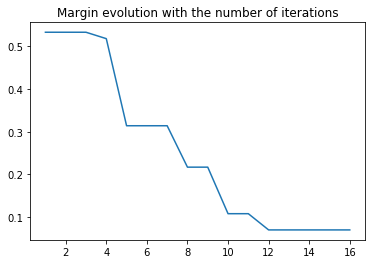
\includegraphics[scale=0.5]{Margin_convergence.png}\\[10pt]
\end{center}
We also plugged in a few other features(using their centroids as arbitrary binary cutoffs) and studied the direction of their weights as learned by the IRL problem. The weights learned by the IRL problem seemed to match our intuition. For instance, it learned a negative weight for SOFA score, negative weight for age which make sense as high SOFA and high age are correlated with death.
In this process, we identified few problems and fixed a large portion of them.
\begin{enumerate}
\item Choice of terminal rewards - In this problem, we are setting the L2 norm of our weight vectors to 1 as we choose the unit vector orthonormal to SVM hyperplane in each iteration. This constraint implicitly ensures that any intermediate state does not have a reward greater than $\sqrt{n_f}$ where $n_f$ is the number of features that we have chosen in the problem. Hence, logic dictates that we have final rewards in absolute magnitude greater than $\sqrt{n_f}$. We ran our IRL problem and found that our intermediate rewards never cross [+6,-6] for using all the 40 odd features. 
\item Epsilon Greedy Solution - We encountered another issue while solving the MDP. Because of the presence of intermediate rewards and a $\gamma$ value, we saw the greedy optimal policy, at times led to us potentially getting us stuck in a loop for a long time. The reason why MDP learned these actions is because the terminal rewards have a strong influence on the solution and hence, the solution tries to delay the inevitable in case of negative rewards though we are not sure if it is clinically possible to oscillate along these states multiple times. To get around this issue, we are adding an $\epsilon$ greediness to the MDP solution. Tuning the $\epsilon$ has been added to our to-do list in the coming days.
\item Loose convergence - This problem currently seems to be the biggest roadblock to the project. IRL algorithm is not strictly converging but rather seems to be loosely converging. If we are to offer a guarantee on the algorithm's final convergence to the expert's features, we need to ensure(both theoretically and practically) that the algorithm strictly provides an infinitesimal improvement in convergence with each step. As we can see from the earlier plot, not each iteration leads our solution towards better convergence though the overall solution eventually converges.  We are trying to infer reasons as to why we are not able to produce more optimal solutions in each increasing step.
\item Simulation Speed - The expert features and the current trajectory features are learned through Monte Carlo Simulations of trajectories. Across 750 states, running 1000 odd simulations for each state makes the program clumsy and takes a long time to optimize. We are thinking of effective use of vectorized operations to solve MDP problems and might rely on parallel MC simulations to make the effective run time faster.
\item Non optimal expert - In this particular state action space definition, the physician policy does not seem to be the most optimal and hence, at times we face the issue of our candidate learners learning arbitrarily better features than the expert causing SVM margins with linear kernels to break as there are learned candidate solutions which are better and worse than the expert simultaneously. If the final goal is understanding the physician policy better, we are planning to stop at the first arrival of a feature within an $\epsilon$ radius adjacent to the physician feature expectations.
\end{enumerate}
\end{itemize}
\section{Next Steps and Milestones}
As we can see in Section \ref{results}, the idea seems to offer promise and lots of scope for further enhancements. Along the direction of feature engineering, the next step is to create one-hot encodings for binary features based on expert advice. Then ,based on the correlation patterns studied earlier, we can incrementally add features and study the optimal features that are perceived to be relevant by clinicians. We have already outlined the issues faced during IRL implementation in Section \ref{results}. We will channelize our efforts into rectifying these issues so that we have a fully functional apprenticeship learning setup for intermediate rewards. \\[10pt]
Once we are successful in deploying the apprenticeship learning framework, we are planning to focus along the following dimensions in a chronological fashion.
\begin{enumerate}
\item Better State Space representations - Collaborate with Cam and Seb's groups
\item Physician/Patient styles - Since the IRL framework largely depends on the expert policy, using EM to understand multiple models of patient/physician styles will be extremely relevant to our use case. Similar to one of the recent papers read in class, we can explore to see the multi-modal nature of this dataset and learn separate IRL weights for each modes. This process would also benefit a lot from a definition of better physician policy.
\item Stochastic policies - We have adopted a purely greedy optimal policy as part of this problem. Recent advances in the amount of data available has triggered lot of research in IRL with stochastic optimal policies. The actions are taught to the agent as a distribution instead of point estimates. This approach is extremely relevant to cases like Sepsis and can implicitly capture the uncertainty around expert actions. 
\end{enumerate}
\textbf{Timelines} - We expect to fully develop the complete apprenticeship learning algorithm in the next two weeks(~November 20) and spend the last 10 days in one or more of the advancements proposed in this section. As we learned from the last checkpoint till now, we can be fazed by several unknown unknowns while solving this problem and hence we might want to get ahead of the problem with a minimal solution at the earliest possible time.

% Acknowledgements should go at the end, before appendices and references

\acks{Most pieces of the approach outlined in this proposal is based on [1]. We will use several components of the research demonstrated in this work for the purpose of this project.}

% Manual newpage inserted to improve layout of sample file - not
% needed in general before appendices/bibliography.

\section*{References}
\begin{enumerate}
\item Abbeel, P., Ng, A.Y.: Apprenticeship learning via inverse reinforcement learning. In: Proceedings of ICML 2004. (2004)
\item Ng, A.Y., Russell, S: Algorithms for inverse reinforcement learning. In: Proceedings of the $17^{th}$ International Conference on Machine Learning (ICML 2000). (2000) 663-670
\item Asoh, H. et.al. : An Application of Inverse Reinforcement Learning to Medical Records of Diabetes Treatment
\item Komorowski, M. et.al. : Continuous State-Space Models for Optimal Sepsis Treatment - A Deep
Reinforcement Learning Approach. arXiv:1705.08422v1 (2017)
\item Dimitrakakis, C., Rothkopf, C.A.: Bayesian multitask inverse reinforcement learning. arXiv:1106.2655v2 (2011)
\item Ramachandran D., Amir E. : Bayesian Inverse Reinforcement Learning, In proceedings of the 20th International Joint Conference on Artificial Intelligence. (2007)
\end{enumerate}



\end{document}